\documentclass{beamer}

\usepackage{cmap}				% To be able to copy-paste russian text from pdf
\usepackage[T2A]{fontenc}
\usepackage[utf8]{inputenc}
\usepackage[russian]{babel}
\usepackage{textpos}
\usepackage{ragged2e}
\usepackage{amssymb}
\usepackage{ulem}
\usepackage{tikz}
\usepackage{pgfplots}
\usepackage{color}
\usepackage{cancel}
\usepackage{multirow}
\pgfplotsset{compat=1.17}
\usetikzlibrary{arrows,snakes,backgrounds,shapes}
\usepgfplotslibrary{groupplots,colorbrewer,dateplot,statistics}
\usepackage{animate}

\usepackage{amsfonts}
\usepackage{amsmath}
\usepackage{amssymb}
\usepackage{graphicx}
\usepackage{setspace}
\usepackage{tabularx}

\usepackage{enumitem}
\setitemize{label=\usebeamerfont*{itemize item}%
  \usebeamercolor[fg]{itemize item}
  \usebeamertemplate{itemize item}}

% remove navigation bar
\setbeamertemplate{navigation symbols}{}

\setbeamertemplate{page number in head/foot}[totalframenumber] 

\usepackage{eurosym}
\renewcommand{\EUR}[1]{\textup{\euro}#1}

\title{Credit valuation adjustment (CVA)}
\author{Артём Бакулин}
\date{11 апреля 2022 г.}

\usetheme{Warsaw}
\usecolortheme{beaver}

\newcommand{\ru}[1]{\begin{otherlanguage}{russian}#1\end{otherlanguage}}
\newcommand{\en}[1]{\begin{otherlanguage}{english}#1\end{otherlanguage}}
\newcommand{\ruen}[2]{#1 (\en{#2})}

% https://tex.stackexchange.com/questions/98003/filter-rows-from-a-table
\pgfplotsset{
    discard if not/.style 2 args={
        x filter/.code={
            \edef\tempa{\thisrow{#1}}
            \edef\tempb{#2}
            \ifx\tempa\tempb
            \else
                \def\pgfmathresult{inf}
            \fi
        }
    }
}



\begin{document}

\begin{frame}
\titlepage
\end{frame}




\begin{frame}{Кредитный риск}
\justify
Торговля внебиржевыми деривативами несёт неизбежный кредитный риск. Если клиент разорится, вы не получите платежей, на которые вы рассчитывали, и окажетесь в убытке.

\vspace{\baselineskip}
Соглашение о залоге (credit support annex, CSA) позволяет снизить риски, обязав стороны сделки на случай своего банкротства оставлять в залог деньги или ценные бумаги, равные по стоимости текущему PV сделки. Кредитный риск трансформируется в другие виды риска (риск ликвидности, юридический риск).

\vspace{\baselineskip}
Решает ли CSA все проблемы? Нет!
\end{frame}

\begin{frame}{CSA в реальном мире}
\justify
Идеальных CSA с непрерывным расчётом залога не существует.
\begin{itemize}
\justifying
\item Периодичность перерасчёта залога и платежей --- в лучшем случае ежедневно.
\item Ограничения на сумму платежей --- CSA threshold, minimal transfer amount (MTA).
\item Margin period of risk: клиент может разориться и не перечислить очередной транш залога, но мы ещё несколько дней (или недель) можем считать это операционным сбоем, а не дефолтом.
\item Многие клиенты либо не имеют (и вряд ли будут) иметь CSA, либо подписывают односторонний CSA (мы платим залог, они --- нет).
\end{itemize}
\end{frame}



\begin{frame}{Credit Valuation Adjustment}
\justify
Credit valuation adjustment, CVA --- поправка к текущей стоимости (PV) дериватива, равная математическому ожиданию потерь от возможного дефолта контрагента в будущем.

\vspace{\baselineskip}
Насколько это важно?
\begin{itemize}
\item Котировка форварда EUR/USD на 1 год на \euro 1\,000\,000: 1.24850 / 1.24862.
\item Виртуальная прибыль банка (половина спрэда): \alert{$+\$60$}.
\item Волатильность EURUSD 9\%, клиент с рейтингом BBB.
\item CVA: \alert{$-\$110$}. Сделка убыточна в момент заключения!
\end{itemize}

\vspace{\baselineskip}
Стандарты финансовой отчётности (МСФО, US GAAP) требуют оценивать деривативы с учётом CVA.
\end{frame}



\begin{frame}{От чего зависит CVA?}
\justify
ООО <<Рога и копыта>> должно выплатить нам \euro1\,000\,000 через год. Как оценить наш CVA?
\begin{itemize}
\justifying
\item Exposure at default (EAD), Expected positive exposure (EPE) --- чем мы рискуем в случае дефолта? \euro1\,000\,000.
\item Default probability (PD) --- какова вероятность, что они разорятся в течение года? Допустим, 1\%.
\item Recovery rate (RR) --- сколько процентов долга мы вернём, продав их имущество (компьютеры и вертолёт CEO)? Предположим, 40\%.
\end{itemize}

Итого наш CVA:
\begin{equation*}
CVA = - (1-RR) \cdot PD \cdot EPE = -(1-40\%) \cdot 1\% \cdot 1\,000\,000 = -6\,000
\end{equation*}
\end{frame}



\begin{frame}{CVA для дериватива}
\justify
Формула CVA дериватива лишь ненамного сложнее формулы для простого долга (*).
\begin{equation*}
CVA = - (1-RR)\int\limits_{0}^{T} p(t)EPE(t)dt
\end{equation*}
$p(t)$ --- вероятность дефолта в момент $t..t+dt$.

$EPE(t)$ --- мат. ожидание потерь от дефолта в момент $t$.

\vspace{\baselineskip}
(*) При условии, что кредитное качество контрагента не имеет корреляции с динамикой базового актива дериватива.
\end{frame}



\begin{frame}{CVA для дериватива}
\justify
План действий:
\begin{itemize}
\justifying
\item Предположить будущее распределение цен базового актива для моментов времени $t_1$, $t_2$, ..., $t_n$.
\item На основе этого вычислить распределение будущих значений $PV$ сделки.
\item Вычислить математическое ожидание (exposure at default)
\item Вычислить вероятности дефолта в интервалы $(0, t_i)$.
\item ...
\item PROFIT!!!
\end{itemize}

Метод Монте-Карло позволяет не выписывать решение аналитически (что может быть сложно или даже невозможно), а получить достаточно хорошее приближение при помощи случайной выборки.
\end{frame}



\begin{frame}{Пример: валютный форвард}
\begin{itemize}
\justifying
\item Мы продали клиенту валютный форвард EUR/USD размером \euro500\,000, сроком на 4 года, по честной рыночной цене.
\item Годовая волатильность пары EUR/USD 9\%. Спот-курс 1.15.
\item Вероятность дефолта клиента 2\% в год, recovery rate 20\%.
\item Процентные ставки, волатильность и вероятность дефолта постоянны. Единственная случайная величина --- курс EUR/USD.
\end{itemize}

\justify
\vspace{\baselineskip}
Важно: эти входные данные следуют из котировок валютного рынка и рынка кредитных свопов (CDS).
\end{frame}



\begin{frame}{Шаг 1: будущие значения спот-курса}
\begin{figure}
\centering
  \makebox[\textwidth]{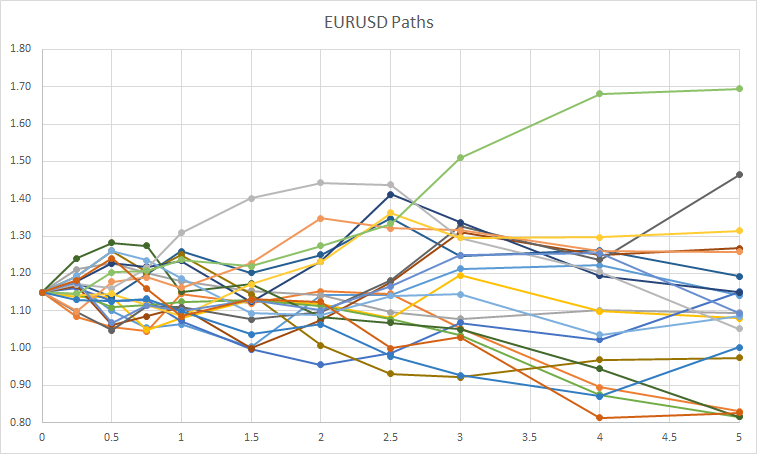
\includegraphics[width=\textwidth]{cva_eurusd_paths.png}}
\end{figure}
\end{frame}



\begin{frame}{Шаг 2: будущие значения PV сделки}
\begin{figure}
\centering
  \makebox[\textwidth]{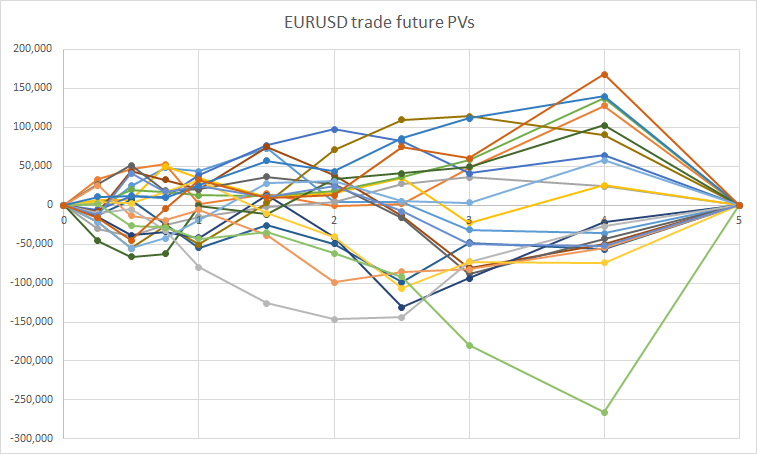
\includegraphics[width=\textwidth]{cva_eurusd_trade_pvs.png}}
\end{figure}
\end{frame}



\begin{frame}{Шаг 3: MAX(0, PV)}
\begin{figure}
\centering
  \makebox[\textwidth]{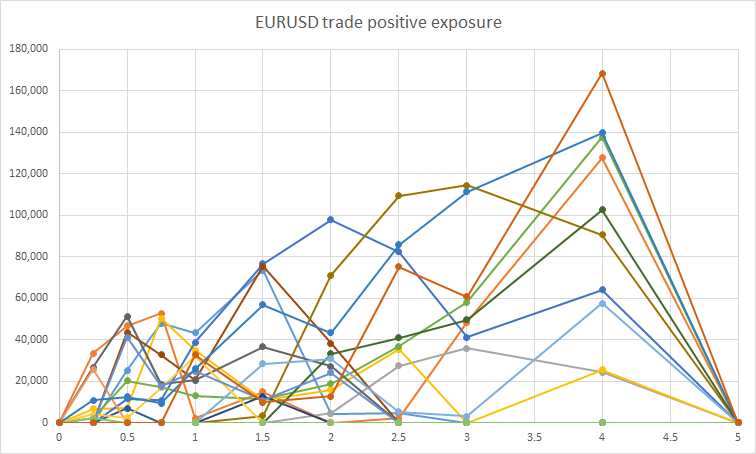
\includegraphics[width=\textwidth]{cva_eurusd_trade_positive_pvs.png}}
\end{figure}
\end{frame}



\begin{frame}{Шаг 4: Expected exposure}
\begin{figure}
\centering
  \makebox[\textwidth]{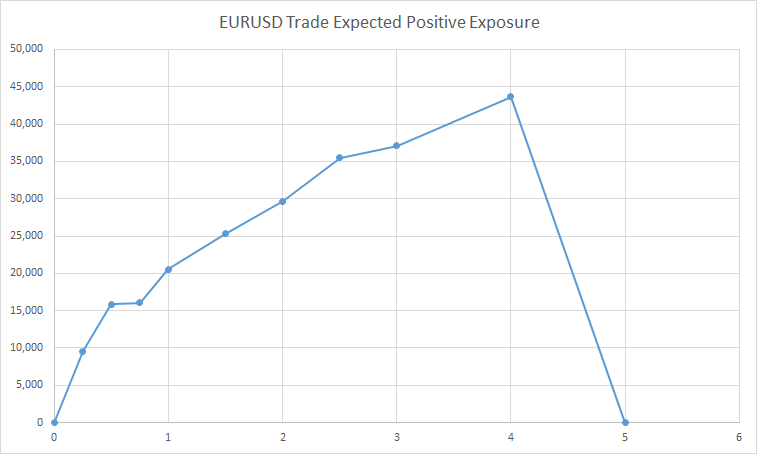
\includegraphics[width=\textwidth]{cva_eurusd_trade_epe.png}}
\end{figure}
\end{frame}



\begin{frame}{Шаг 5: Складываем всё вместе}
\begin{tabular}{l|l|l|l|l|l}
Time & Surv. Prob. & Def. Prob. & EPE & Loss & Exp. Loss \\
 \hline
0		& 100.0\%	& 0.00\%	& \euro0		& \euro0		& \euro0 \\
0.25	& 99.5\%	& 0.50\%	& \euro9\,578	& \euro7\,662	& \euro38 \\
0.5		& 99.0\%	& 0.50\%	& \euro15\,881	& \euro12\,705	& \euro63 \\
0.75	& 98.5\%	& 0.49\%	& \euro16\,059	& \euro12\,847	& \euro63 \\
1		& 98.0\%	& 0.49\%	& \euro20\,545	& \euro16\,436	& \euro81 \\
1.5		& 97.0\%	& 0.98\%	& \euro25\,289	& \euro20\,231	& \euro197 \\
2		& 96.1\%	& 0.97\%	& \euro29\,657	& \euro23\,725	& \euro229 \\
2.5		& 95.1\%	& 0.96\%	& \euro35\,519	& \euro28\,415	& \euro272 \\
3		& 94.2\%	& 0.95\%	& \euro37\,105	& \euro29\,684	& \euro281 \\
4		& 92.3\%	& 1.86\%	& \euro43\,667	& \euro34\,933	& \euro651 \\
5		& 90.5\%	& 1.83\%	& \euro0		& \euro0		& \euro0 \\
\hline
\multicolumn{5}{r}{CVA:} & \euro1\,876
\end{tabular}
\end{frame}



\begin{frame}{Что если мы добавим ещё сделку?}
\justify
Тот же самый клиент заключает новую сделку:
\begin{itemize}
\item Клиент продаёт форвард GBP/USD, на 425\,000 GBP, сроком на 3 года.
\item Курс GBP/USD 1.35, годовая волатильность 8\%.
\end{itemize}

\vspace{\baselineskip}
Важное дополнение: волатильность кросса EUR/GBP 7\%, следовательно корреляция курсов EUR/USD и GBP/USD равна 0.67.
\end{frame}



\begin{frame}{Шаг 1: будущие значения спот-курса}
\begin{figure}
\centering
  \makebox[\textwidth]{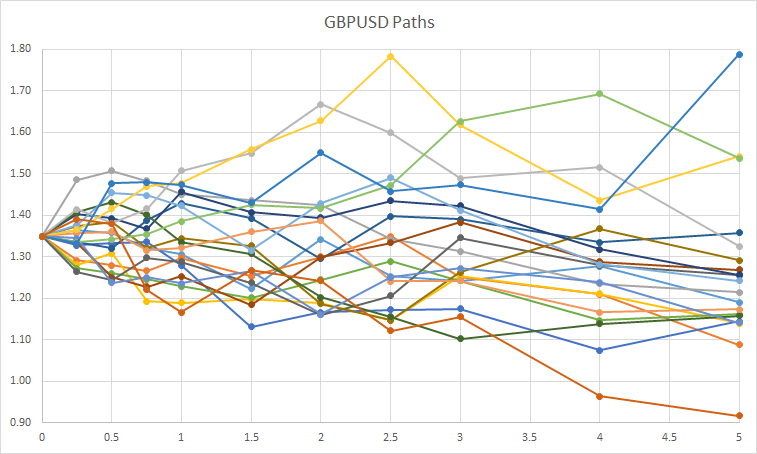
\includegraphics[width=\textwidth]{cva_gbpusd_paths.png}}
\end{figure}
\end{frame}



\begin{frame}{Шаг 2: будущие значения PV сделки}
\begin{figure}
\centering
  \makebox[\textwidth]{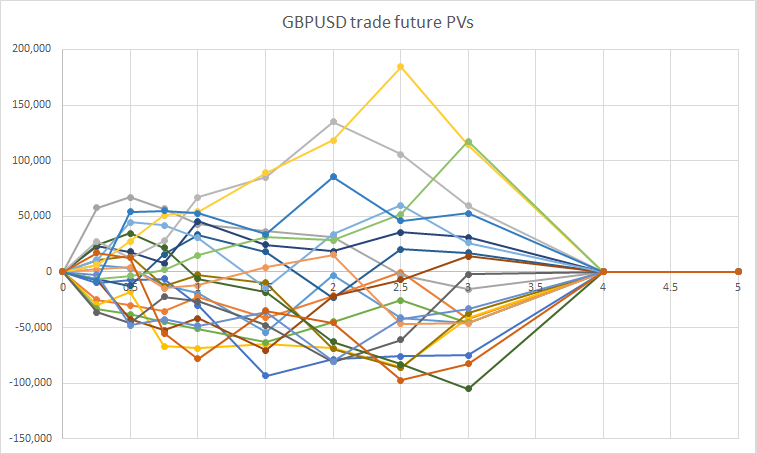
\includegraphics[width=\textwidth]{cva_gbpusd_trade_pvs.png}}
\end{figure}
\end{frame}



\begin{frame}{Шаг 2Б: будущие значения PV портфеля}
\begin{figure}
\centering
  \makebox[\textwidth]{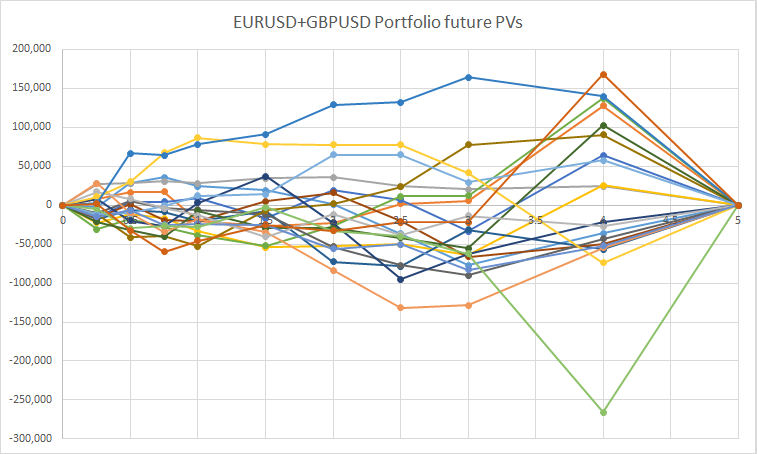
\includegraphics[width=\textwidth]{cva_portfolio_pvs.png}}
\end{figure}
\end{frame}



\begin{frame}{Шаг 3: MAX(0, PV)}
\begin{figure}
\centering
  \makebox[\textwidth]{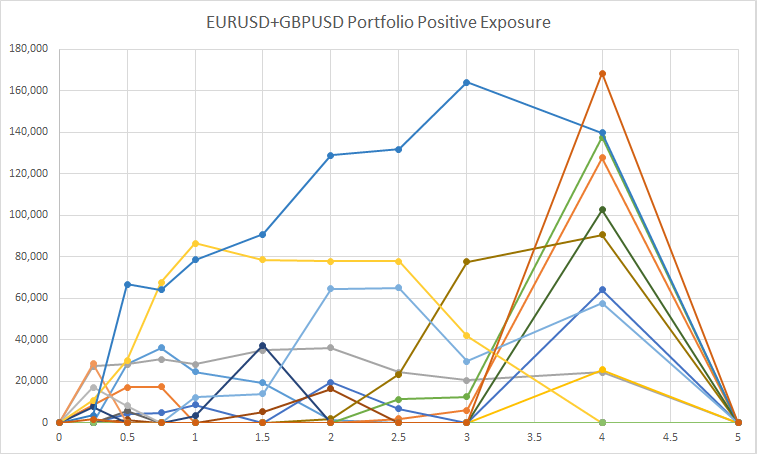
\includegraphics[width=\textwidth]{cva_portfolio_positive_pvs.png}}
\end{figure}
\end{frame}



\begin{frame}{Шаг 4: Expected exposure}
\begin{figure}
\centering
  \makebox[\textwidth]{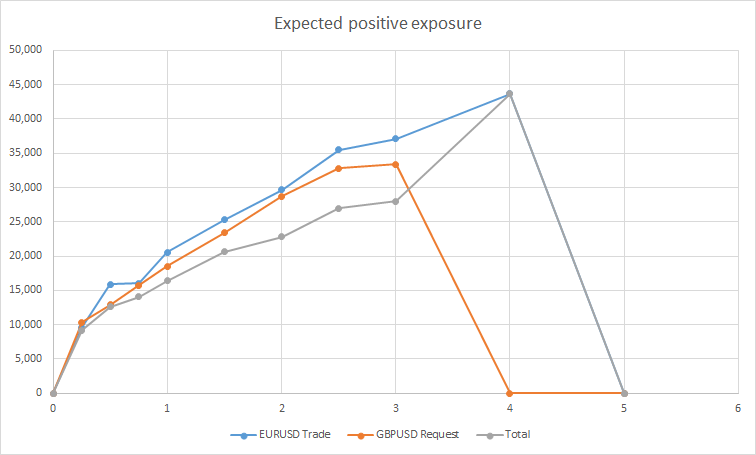
\includegraphics[width=\textwidth]{cva_portfolio_epe.png}}
\end{figure}
\end{frame}



\begin{frame}{Шаг 5: Складываем всё вместе}
\begin{tabular}{l|l|l|l|l|l}
Time & Surv. Prob. & Def. Prob. & EPE & Loss & Exp. Loss \\
 \hline
0		& 100.0\%	& 0.00\%	& \euro 0			& \euro 0			& \euro 0 		\\
0.25	& 99.5\%	& 0.50\%	& \euro 9\,182		& \euro 7\,346		& \euro 37		\\
0.5		& 99.0\%	& 0.50\%	& \euro 12\,568	& \euro 10\,054	& \euro 50		\\
0.75	& 98.5\%	& 0.49\%	& \euro 14\,042	& \euro 11\,234	& \euro 55		\\
1		& 98.0\%	& 0.49\%	& \euro 16\,388	& \euro 13\,111	& \euro 64		\\
1.5		& 97.0\%	& 0.98\%	& \euro 20\,606	& \euro 16\,485	& \euro 161	\\
2		& 96.1\%	& 0.97\%	& \euro 22\,829	& \euro 18\,263	& \euro 176	\\
2.5		& 95.1\%	& 0.96\%	& \euro 26\,986	& \euro 21\,589	& \euro 206	\\
3		& 94.2\%	& 0.95\%	& \euro 28\,006	& \euro 22\,405	& \euro 212	\\
4		& 92.3\%	& 1.86\%	& \euro 43\,667	& \euro 34\,933	& \euro 651	\\
5		& 90.5\%	& 1.83\%	& \euro 0			& \euro 0			& \euro 0		\\
\hline
\multicolumn{5}{r}{CVA:} & \euro1\,613
\end{tabular}
\end{frame}



\begin{frame}{Наблюдения и выводы}
\begin{itemize}
\justifying
\item CVA портфеля не равен сумме CVA отдельных сделок.
\item CVA зависит не только от волатильностей отдельных риск-факторов, но и от корреляций между ними.
\item Чтобы аккуратно посчитать CVA, вам нужно знать ВЕСЬ портфель клиента (включая FX, Rates и Equities).
\item Новая сделка может уменьшить CVA, в этом случае вы можете <<поправить>> bid/ask --- клиент увидит не тот же самый mid, который видят другие клиенты.
\end{itemize}
\end{frame}



\begin{frame}{CVA и риск}
\justify
После того, как сделка заключена, CVA может измениться по любой из следующих причин:
\begin{itemize}
\justifying
\item Изменение PV сделки из-за изменения цены базового актива (<<дельта>>). Больше PV --- больше CVA.
\item Изменение ожидаемой волатильности и корреляций (<<вега>>). Выше волатильность --- больше CVA.
\item Изменение вероятности дефолта (<<CS01>>, credit-spread-01). Обычно, выше вероятность дефолта --- больше CVA.
\end{itemize}

\justify
Недостаточно один раз посчитать CVA перед сделкой. Расчёт CVA является важной частью расчёта прибыли и рисков в конце каждого рабочего дня!
\end{frame}



\begin{frame}{CVA и риск}
\justify
Стандартная практика в крупных банках --- выделять отдельную группу трейдеров (<<деск>>) CVA. Их задача --- расчёт начального CVA и хэджирование с тем, чтобы CVA в будущем не изменялся.

\vspace{\baselineskip}
Методы управления риском:
\begin{itemize}
\justifying
\item Покупка или продажа базового актива --- для хэджирования <<дельты>>.
\item Покупка опционов на базовый актив --- для хэджирования <<веги>>.
\item Покупка CDS либо на отдельного эмитента, либо на индекс --- для хэджирования <<CS01>>.
\item Принятие риска (warehouse) --- иногда дешевле принять кредитный риск, чем хэджировать его.
\end{itemize}
\end{frame}



\begin{frame}{Wrong-way risk}
\justify
Формула для CVA верна только в предположении, что корреляция между кредитным качеством клиента и PV сделки равна нулю. Вообще говоря, это не так.
\begin{itemize}
\justifying
\item Российский банк продал нам годовой форвард на USD/RUB по курсу 70.0.
\item К осени нефть упала до \$30, доллар вырос до 120.
\item Выросла ли вероятность дефолта этого российского банка? Вероятно, да.
\end{itemize}

Это называется wrong-way risk. Мы одновременно получили и выросшую вероятность дефолта, и более высокие ожидаемые потери от дефолта. Этот риск крайне сложно учитывать и моделировать из-за недостатка данных, но полезно о нём помнить.
\end{frame}



\begin{frame}{Debt Valuation Adjustment}
\justify
Если клиент рассуждает так же как мы, то он тоже вычисляет CVA --- поправку на риск дефолта контрагента, то есть нас.

\vspace{\baselineskip}
Debt Valuation Adjustment (DVA) --- зеркальное отражение этого клиентского CVA. Больше CVA клиента (потенциальные убытки) CVA --- больше DVA у нас (если мы разоримся, нам не надо будет платить).

\vspace{\baselineskip}
Согласно МСФО, банки обязаны учитывать DVA, оценивая прибыль по деривативной позиции. Если банк окажется на грани банкротства, мы напоследок увидим огромную прибыль в деривативах (из-за DVA)!
\end{frame}



\begin{frame}{Debt Valuation Adjustment}
\justify
Текущий рыночный консенсус --- учитывать DVA в отчётности, но не вкладывать его в цены и не хэджировать его изменение.

\begin{itemize}
\justifying
\item Вкладывать DVA в цены --- продавать клиентам деривативы дешевле, чем обычно.
\item Хэджировать увеличение DVA --- покупать собственные облигации, либо продавать CDS на себя же.
\item Хэджировать уменьшение DVA --- шортить собственные облигации, покупать CDS на себя же.
\end{itemize}

Маленькое облегчение: считается, что DVA обратно скоррелирован с Funding Valuation Adjustment (FVA), и поэтому можно смириться и не хэджировать его.
\end{frame}


\begin{frame}{Если всего этого мало}
\begin{itemize}
\justifying
\item Capital Valuation Adjustment (KVA).
\item Funding Valuation Adjustment (FVA).
\item Margin Valuation Adjustment (MVA).
\item Collateral Valuation Adjustment (ColVA)
\end{itemize}

\justify
Подробнее: Jon Gregory. The xVA Challenge: Counterparty Credit Risk, Funding, Collateral and Capital. Wiley, 2015.
\end{frame}

\end{document}


